
\chapter{Proposed Framework}
\label{capitulo4}
The framework was idealized to work and different scenarios, in the Section \ref{sub:1} is presented the proposal with one camera with the object calibration. In Section \ref{sub:2} is defined the problem with one camera, but using a known map with some metrics to estimate the position along the map. The Section \ref{sub:3} is defined the approach with multicameras and real-time processing. 



\section{Approach 1 - One camera with object calibration}\label{sub:1}

The first proposed is based on the approach of the authors of the paper \cite{8678911}, where it is necessary to calibrate the camera before start the object recognition and classification. This proposal were defined in six steps, as shown in Figure \ref{fig:proposal1}.

\begin{figure}[H]
\centering
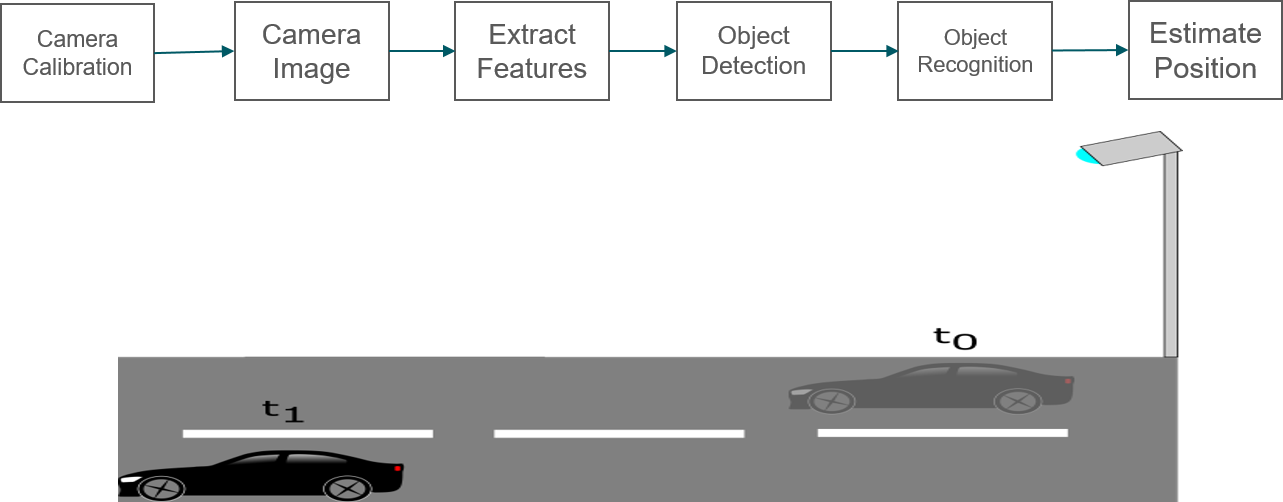
\includegraphics[width=\textwidth]{imagens/proposal1.png}
\caption{Proposal using only one camera with object calibration}
\label{fig:proposal1}
\end{figure}

\subsection{Camera Calibration}

For this task is necessary to reduce the distortion of the camera, the camera used on the tasks has a noise, for this approach is really recommend to perform this step. Following this requirement, a script in Python language with the OpenCV library based in \cite{zhu2020camera} was developed. Furthermore, with calibration you may also determine the relation between the camera’s natural units (pixels) and the real world units (for example millimeters).

Using the intrinsic parameters of the camera, using the in (\ref{eq:calibration}), one point is projected on the image plane. 

Where the 3D point ($X_w, Y_w, Z_w$) in the world coordinates to its projection ($u, v$) in the image image coordinates.


\begin{equation}
    \label{eq:calibration}
    \begin{bmatrix}
        u'
        \\v' 
        \\ z' 
        
        \end{bmatrix} = P \begin{bmatrix}
        X_w\\
        Y_w 
        \\ Z_w
        \\ 1
        
        \end{bmatrix}
\end{equation}

In \ref{eq:points}, $\mathbf{P}$ is a 3x4 projection matrix combined of two different parts, the intrinsic parameters of the camera ($\mathbf{K}$) and the extrinsic matrix ($[\mathbf{R}|t]$) that is based on the combination of 3x3 rotation matrix $\mathbf{R}$ and 3x1 translation $t$ vector. 

\begin{equation}
    \label{eq:points}
    P = \overbrace{\hbox{\boldsymbol{K}}}^{\hbox{Intrinsic Matrix}} x \overbrace{\hbox{[\boldsymbol{R}|t]}}^{\hbox{Extrinsic Matrix}}
\end{equation}

The intrinsic matrix ($\mathbf{K}$) is an upper triangular matrix as shown in (\ref{eq:intrisic}). 

\begin{equation}
    \label{eq:intrisic}
\textbf{K} = \begin{bmatrix}
    f_x & \gamma  & c_x\\ 
    0 & f_y & c_y\\ 
    0 & 0 & 1
    \end{bmatrix}
\end{equation}

where, $f_x, f_y$ are the $x$ and $y$ focal lengths, $c_x, c_y$ are the $x$ and $y$ coordinates of the center in the image plane, $\gamma$ is the skew between the axes, in this master's thesis was defined equal to $0$.  

\subsection{Camera Image}

The image camera model depicted in Figure \ref{fig:image_formation} describes the mathematical relationship between the coordinates of a point in 3-dimension space and its projection onto
the image plane of a camera, where this aperture is described as a point and no lenses are used to focus light. This means that the model can only be used as a first order approximation of the mapping from a 3D scene to a 2D image \cite{forsyth2002computer}.




\begin{figure}[H]
\centering
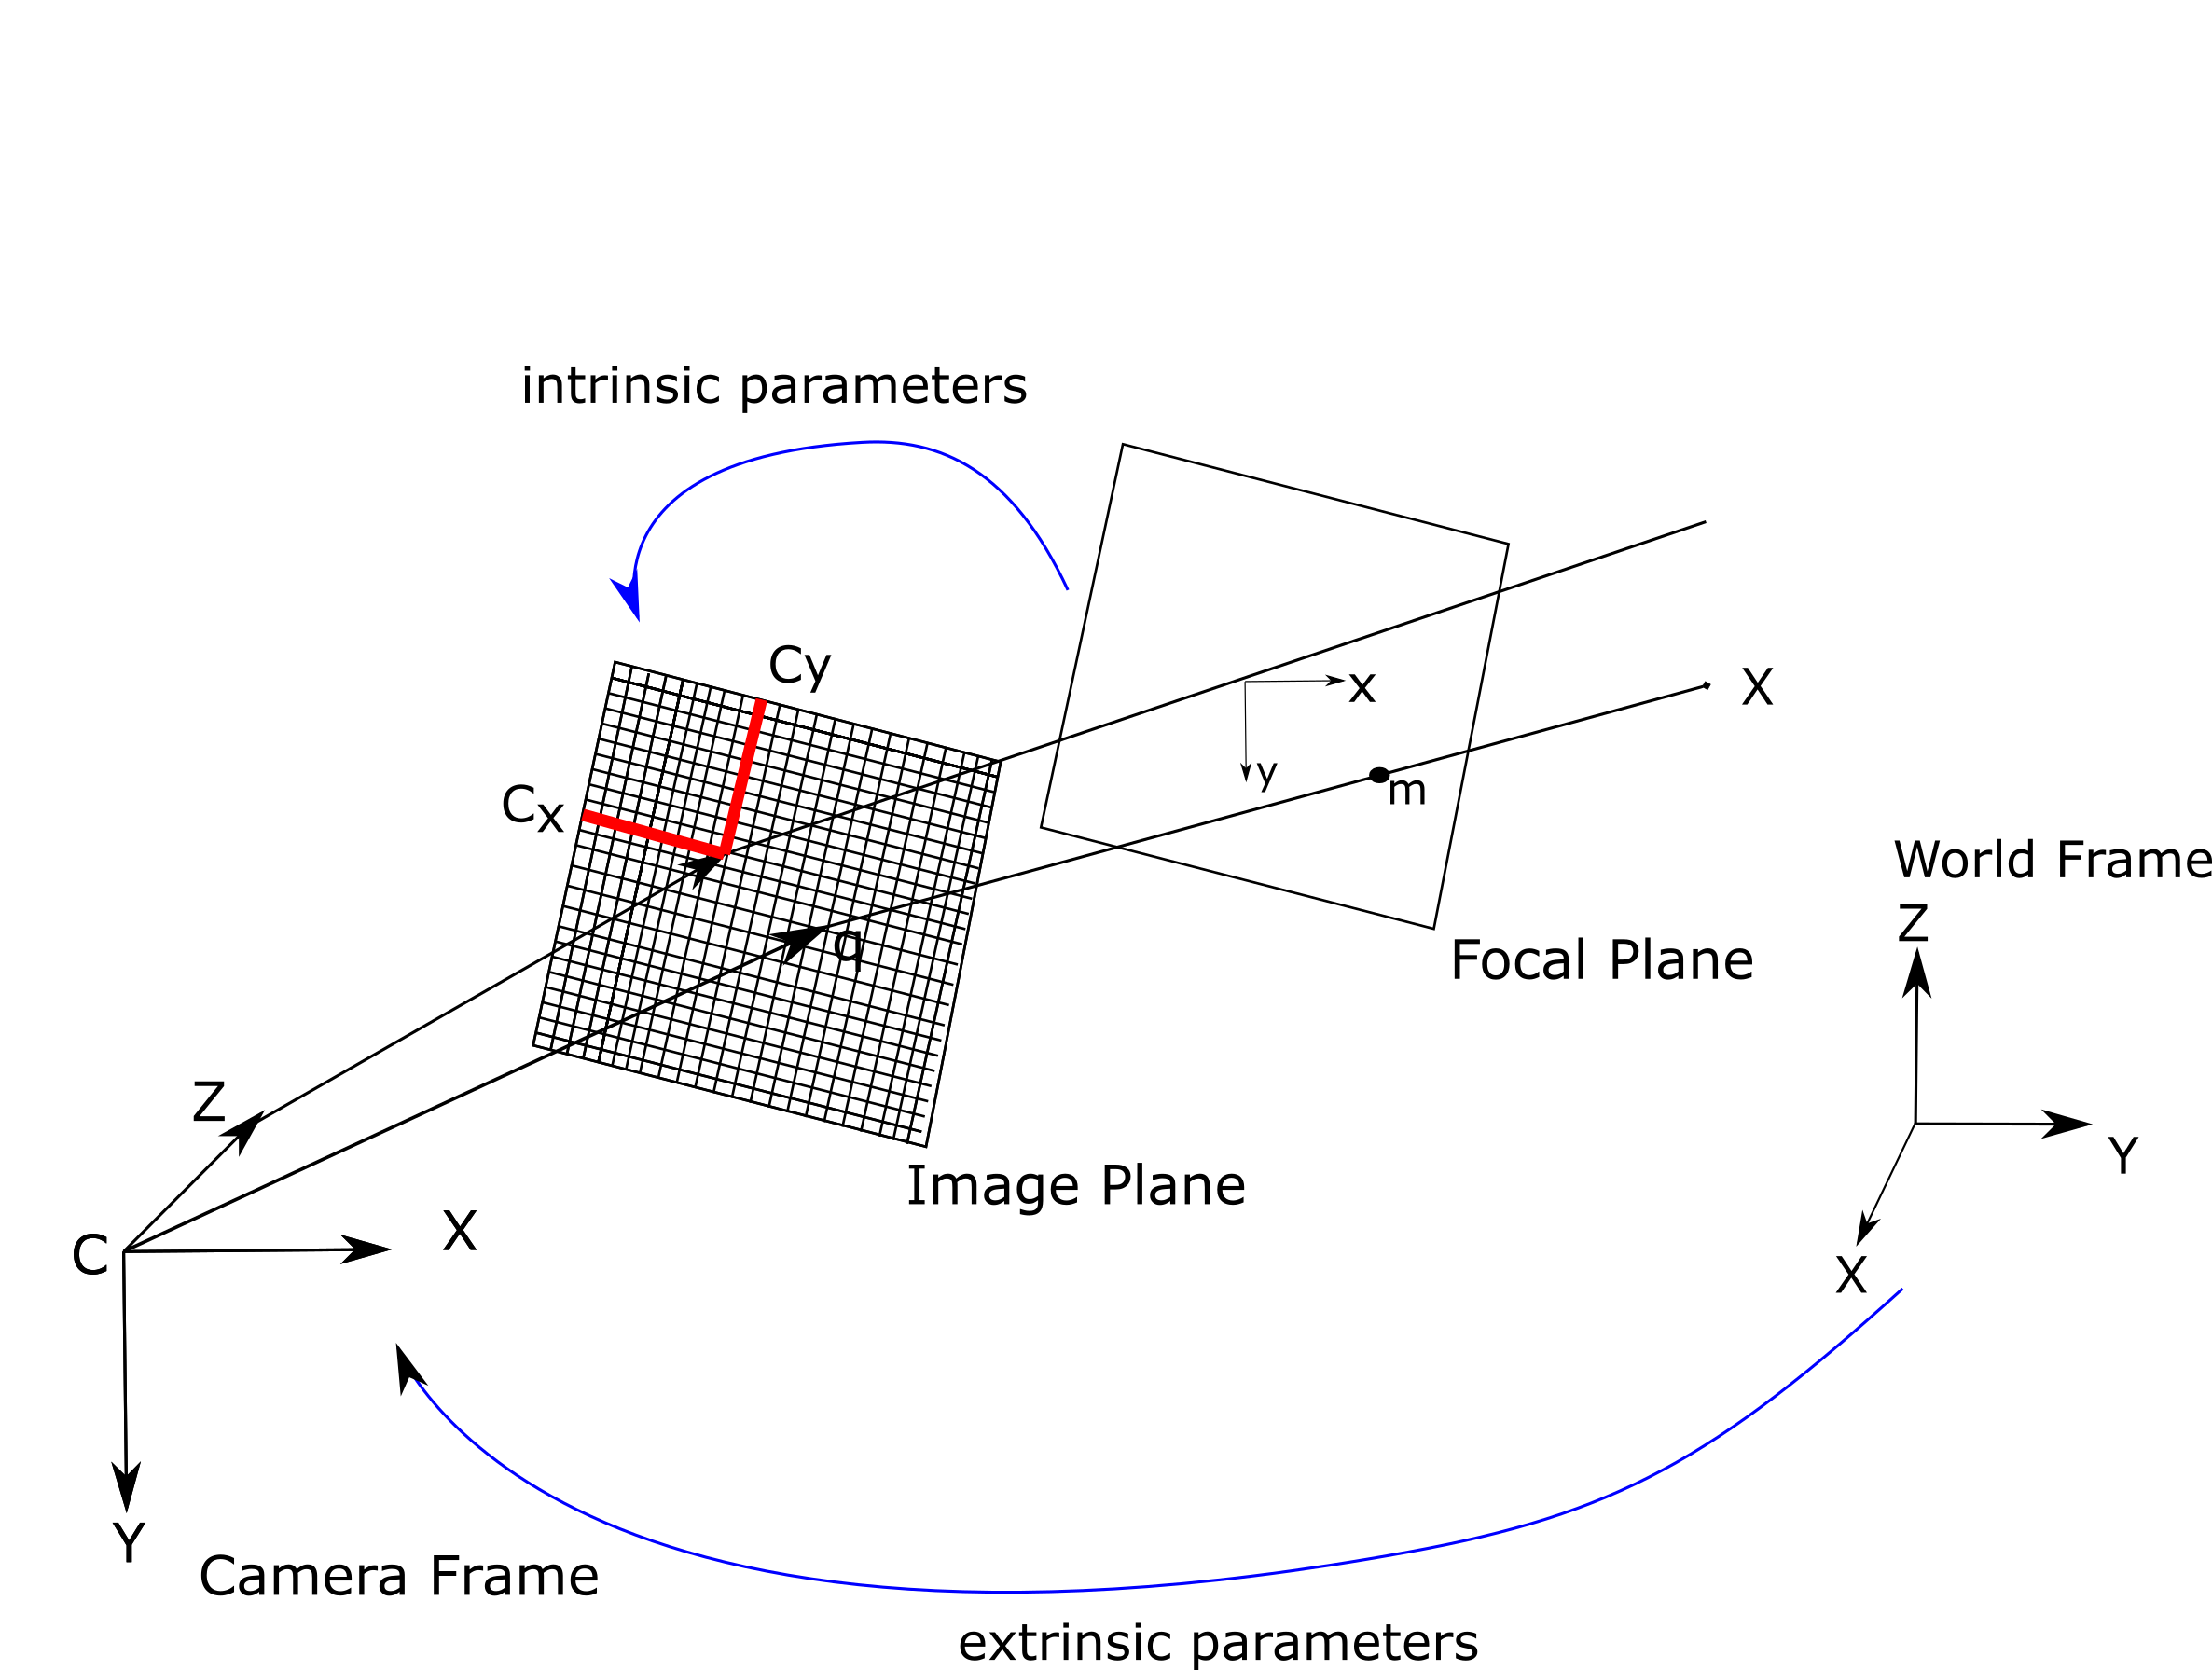
\includegraphics[width=\textwidth]{imagens/image_formation.png}
\caption{The camera model for image formation based on some metrics and known parameters}
\label{fig:image_formation}
\end{figure}

\subsection{Extract Features}

When it is necessary to work with variables that contains many contents, there is a necessity to improve this work and reduce the computer bottleneck during the process. In machine learning (ML), there are variables that are independents or some cases features on which the final output is done. And in other cases that numbers of these features increases it and reduce the ability to visualize the data. 

For example, the image resolution of the collected data for training part of the ML algorithm is $1392$ pixels in height and $512$ pixels in width, for the total $712,704$ pixels in total. Where each pixel has a single pixel-value associated with it, indicating the darkness or lightness of that pixel. The range of these numbers are between $0$ and $255$, and with this premise is necessary to determine which objects the image contains.

The task was performed by feature extraction which is a process to creating a new features from existing features, and with this allows to give more information and less redundancies \cite{wang2019data}.

A mathematical tool called Principal Component Analysis (PCA) was used in this step, and the PCA is used to decompose a multivariate dataset in a set of successive orthogonal components that explain a maximum amount of the variance \cite{pedregosa2011scikit}. In Figure \ref{fig:pca_step1} is shown how the technique works, the data is decomposed into perpendicular vector where the information is unrolled. And with more variance means more information of data.

\begin{figure}[H]
\centering
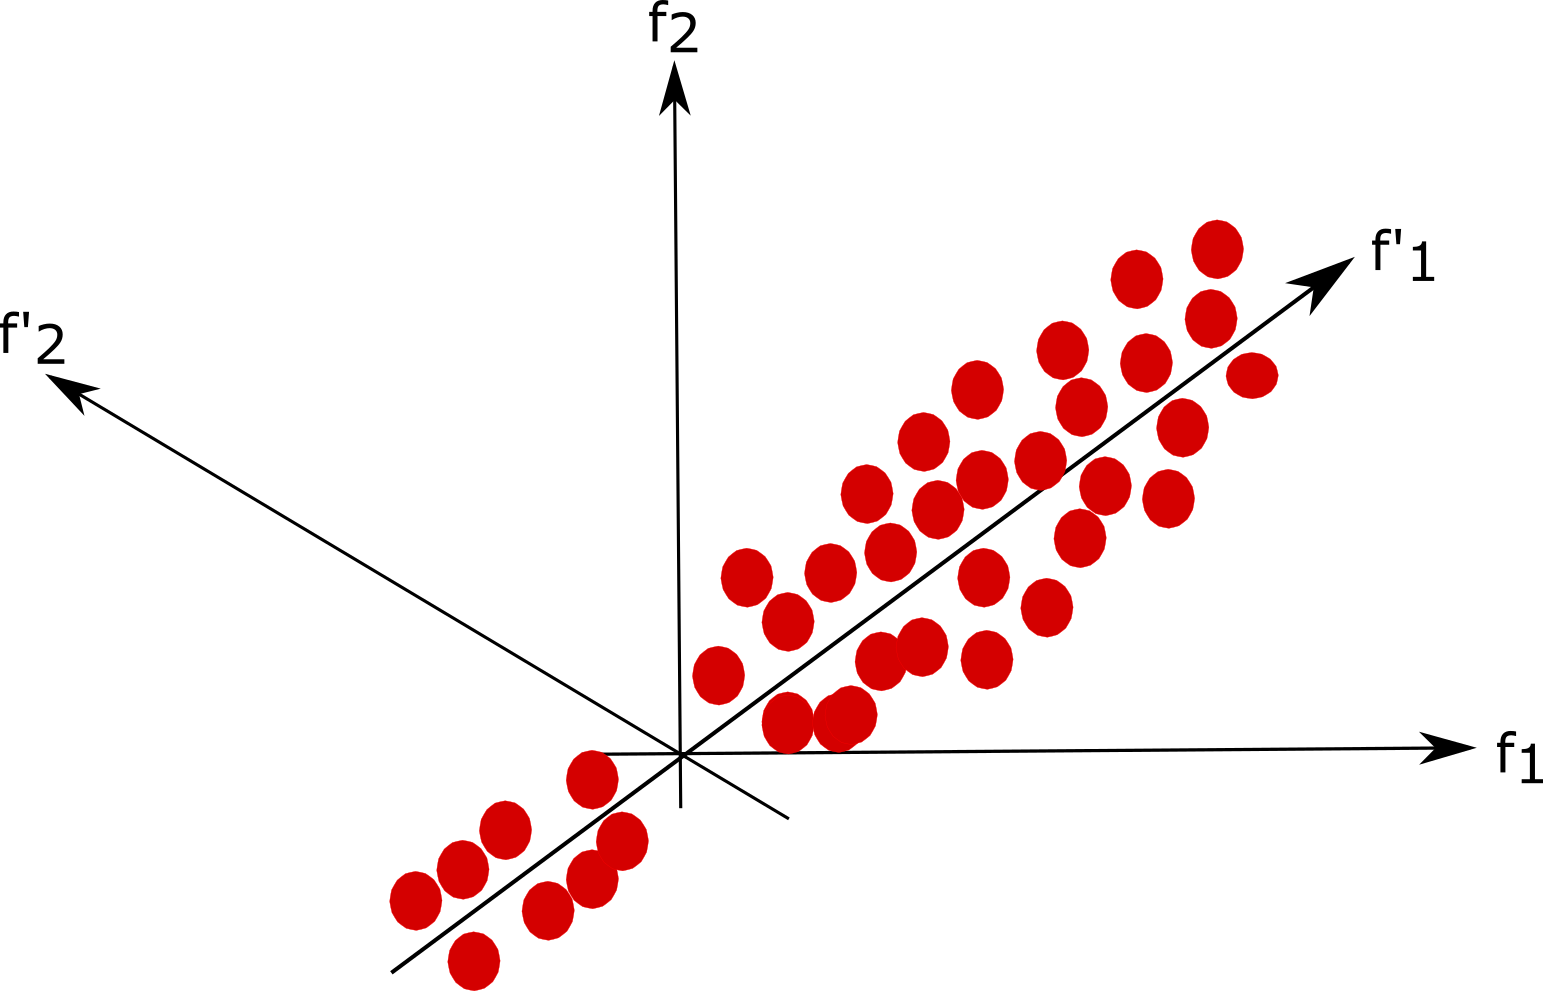
\includegraphics[scale=0.7]{imagens/pca1.png}
\caption{Maximum variance in $f_1'$, where the red circles mean the data points of the data set, $f_1$ is the feature 1 on x-axis, $f_2$ is the feature 2 on y-axis}
\label{fig:pca_step1}
\end{figure}


Based on Figure \ref{fig:pca_step2}, is necessary to find a direction $f_i$ such has the variance of $x_i's$ project on $f_i's$ has the maximum value. Also, it is necessary to rotate the previous axis to find $f_i's$, and finally drop $f_2$

\begin{figure}[H]
\centering
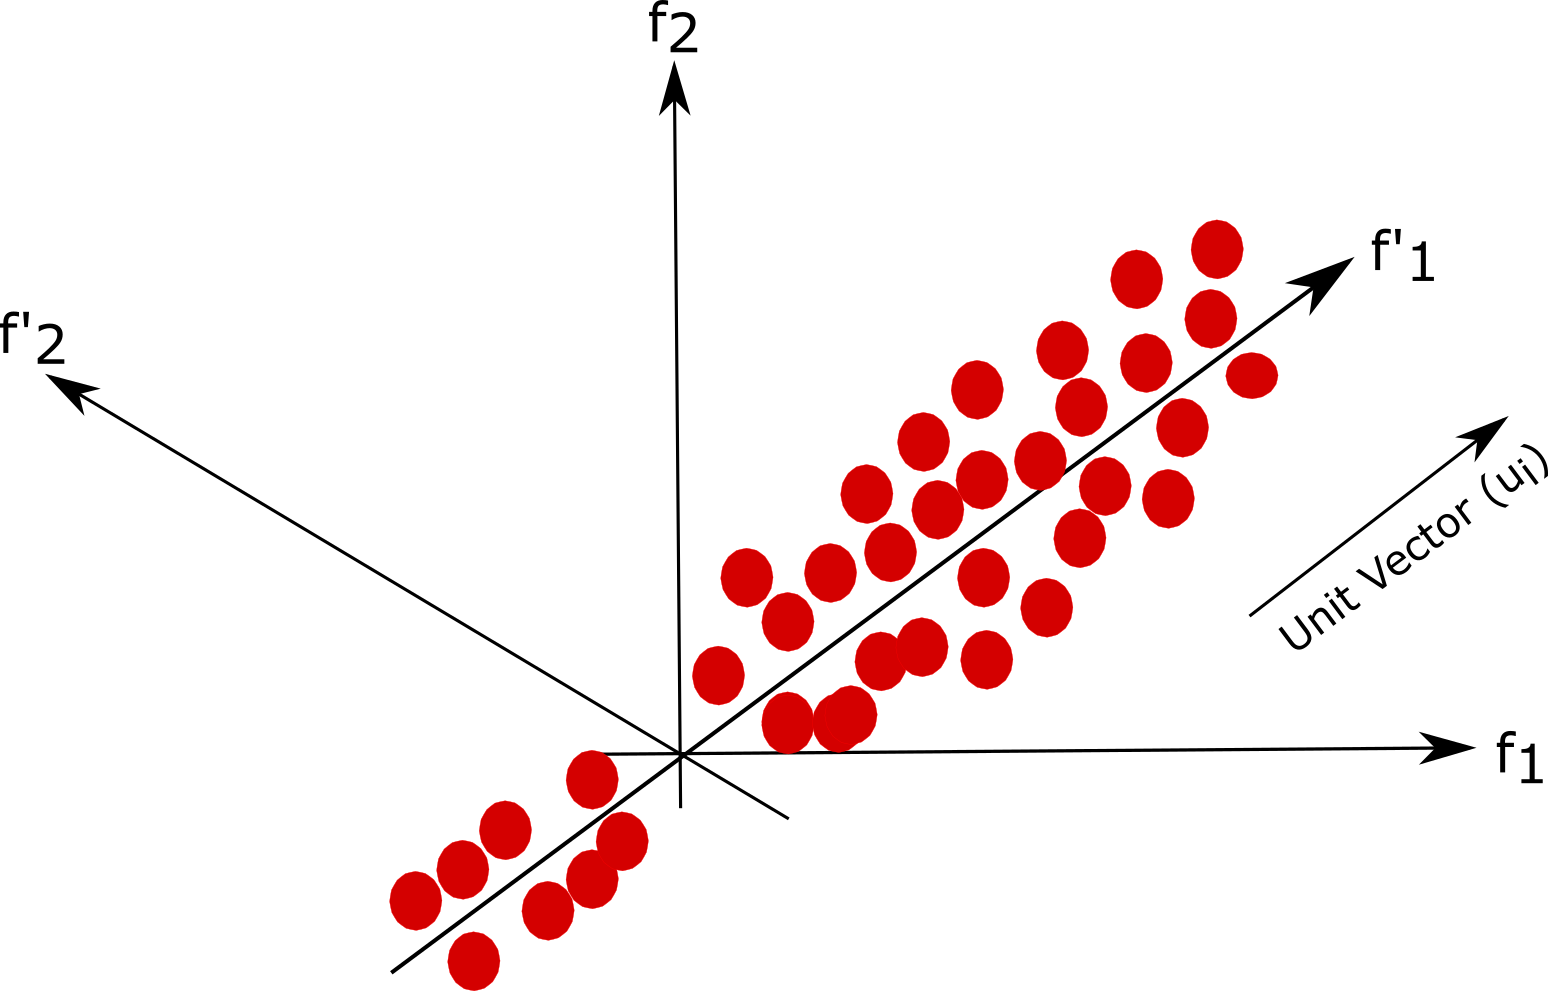
\includegraphics[scale=0.7]{imagens/pca2.png}
\caption{Unit vector direction of maximum variance}
\label{fig:pca_step2}
\end{figure}

So, to find the direction of the $f_i's$ which has the maximum variance, thus, unit vector in the direction of maximum variance = $U_i$, in (\ref{eq:eq_pca}) is described how to compute this distance. 


\begin{subequations}
\begin{equation}
    \label{eq:eq_pca}
    x_i' = \textnormal{Projection of} ~ x_i ~\textnormal{on unit vector} ~u_i
\end{equation}
  
\begin{equation}
  = u_i^Tx_i
\end{equation}

\begin{equation}
    \overline{x_i'} = u_i^T\cdot\underbrace{\overline{x}_i}_{Mean ~ Vector}
\end{equation}
\begin{equation}\label{step_pca}
    var\left \{ u^Tx_i \right \}^n_{i=1} = \frac{1}{n}\sum_{i=1}^{n}\left ( u_i^Tx_i - \underbrace{u_i^T\overline{x}_i}_{Mean~\overline{x}_i} \right )^2
\end{equation}

\end{subequations}

In (\ref{step_pca}) is possible to find out the $u_i$ which gives the maximum variance. And this problem can be defined as distance minimization \cite{liu2004distance}. 

In Figure \ref{fig:pca_step3} the vector which gives the minimum distance $(d_1,d_1, \cdots)$ when $x_i's$ are projected on $u_i$. 

\begin{figure}[H]
\centering
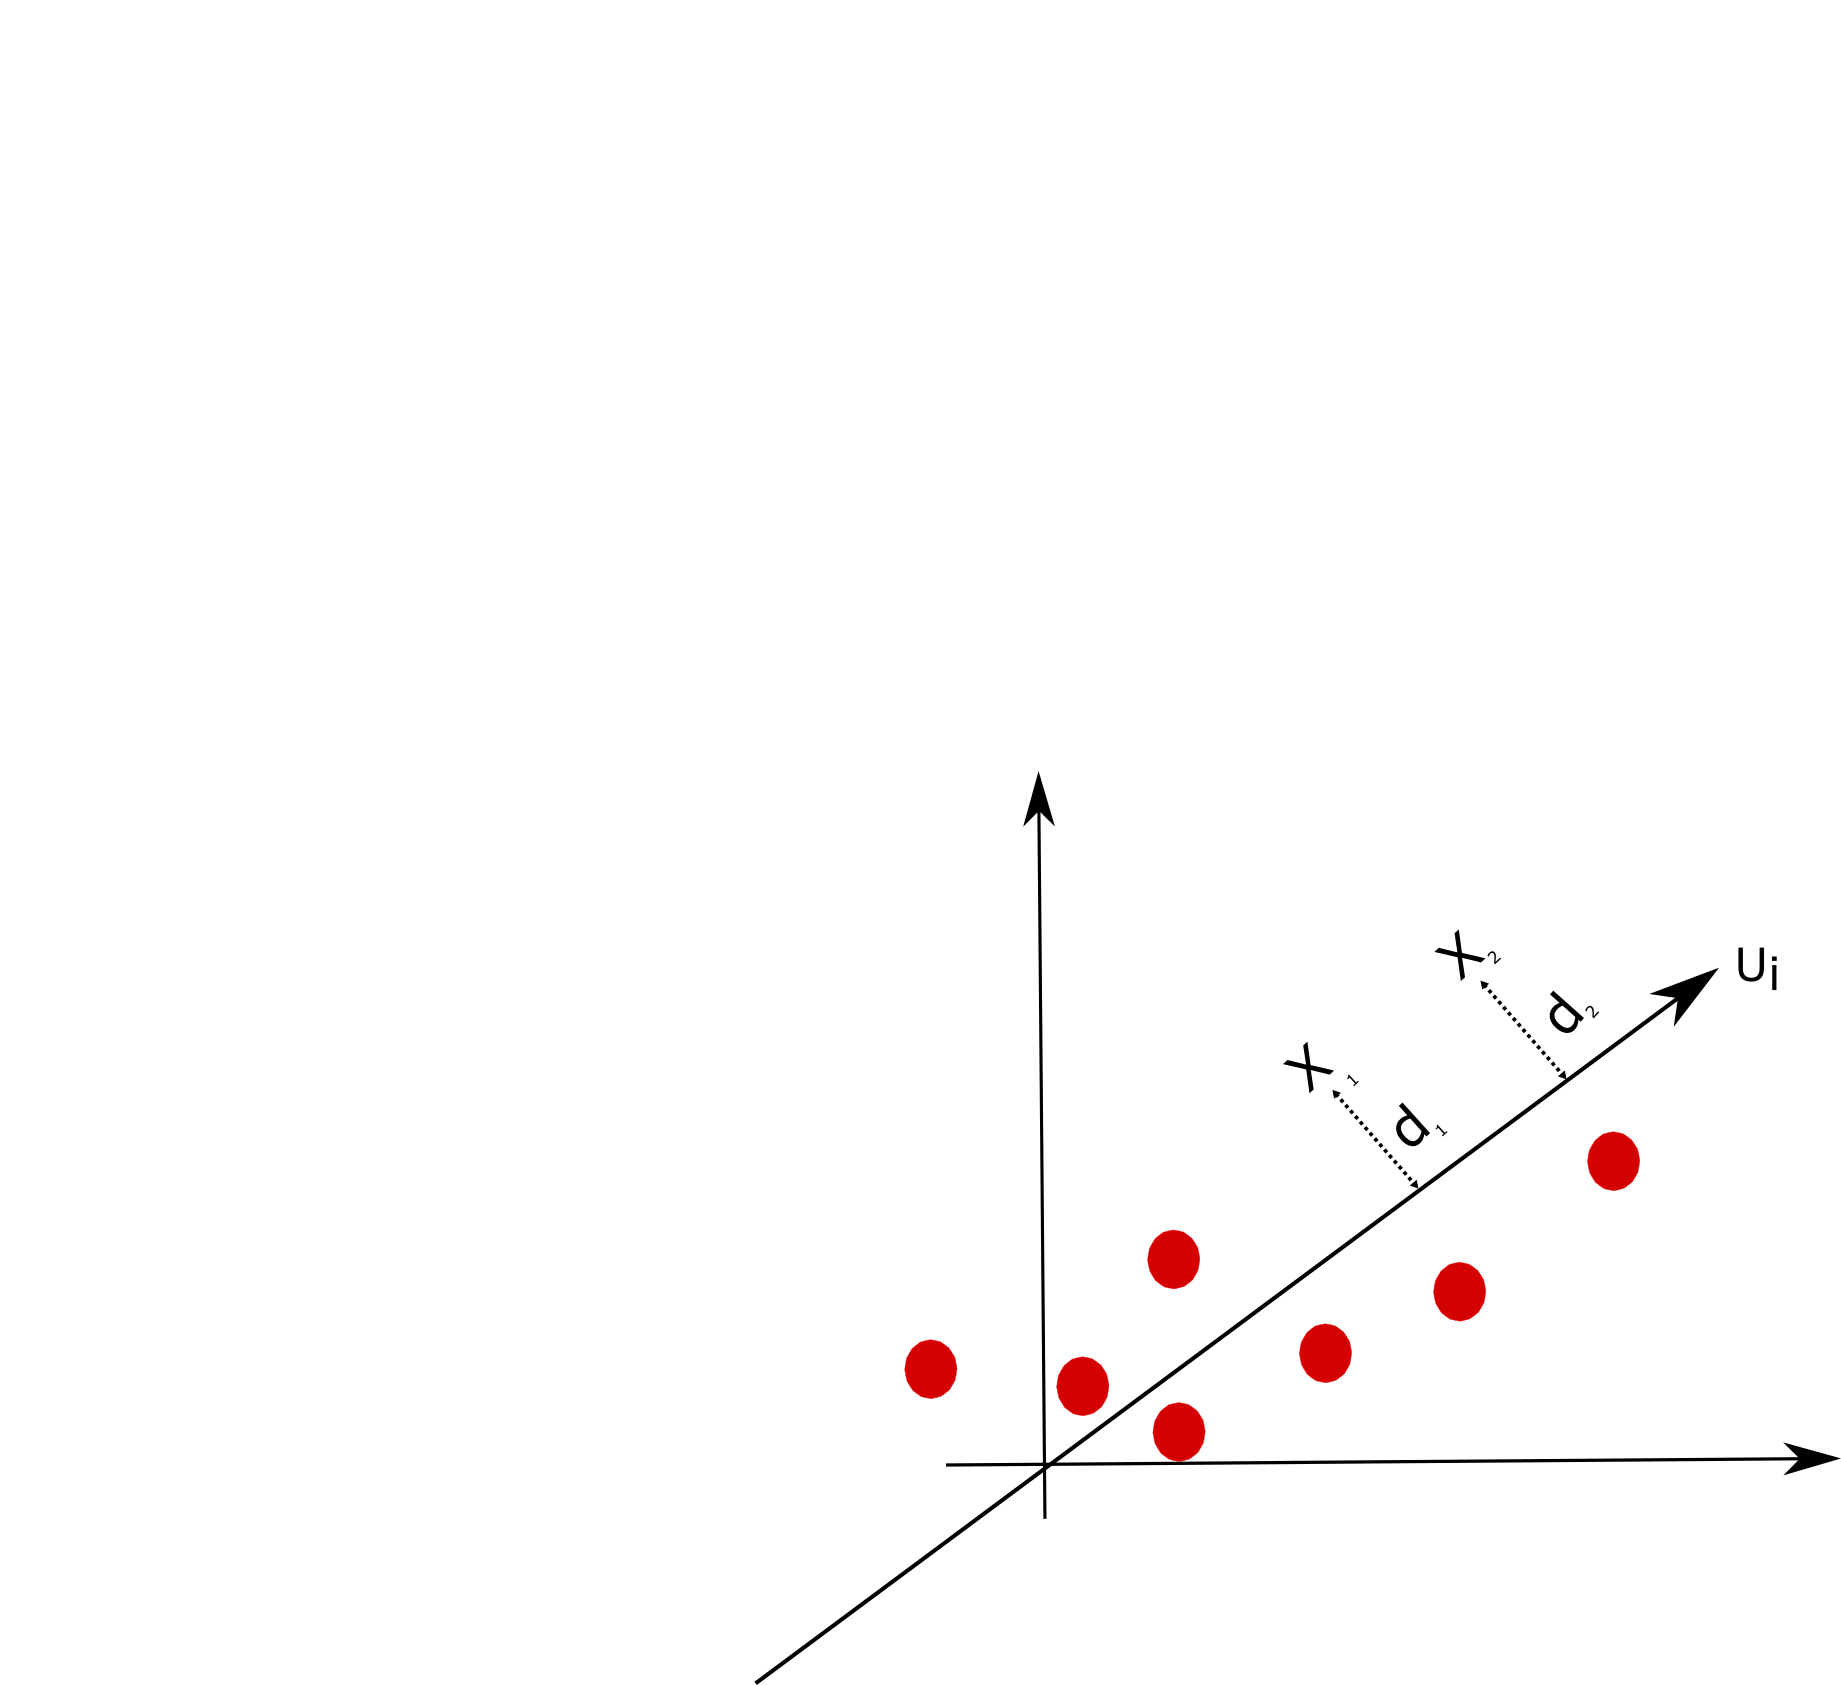
\includegraphics[scale=0.7]{imagens/pca3.png}
\caption{Distance minimization PCA}
\label{fig:pca_step3}
\end{figure}

In (\ref{eq:pca_4}) the equation to finds the vector $u_i$ which gives the minimum distance. 

\begin{subequations}
    \label{eq:pca_4}
    \begin{equation}
        d_i^2 = \left \| x_i \right \|^2 - \left ( u^Tx_i \right )^2
    \end{equation}
    \begin{equation}
        = \left ( x^Tx_i \right ) - (u^Tx_i)^2
    \end{equation}
    \begin{equation}
        min_{u_i} \sum_{i=1}^{n}\left ( x_i^Tx_i - \left ( u^Tx_i \right )^2 \right )
    \end{equation}
\end{subequations}

Solution to above Equations is given by Eigenvalues and Eigenvectors. 

Where, the matrix $\mathbf{X}$ in (\ref{eq:matrix}) is the matrix of the data points with the shape $(n x d)$

\begin{equation}\label{eq:matrix}
    \mathbf{X} = \begin{bmatrix} 
    a_{11} & a_{12} & \dots \\
    \vdots & \ddots & \\
    a_{K1} &        & a_{KK} 
    \end{bmatrix}
\end{equation}

The square symmetric matrix is defined as $S_{dxd} = X^T_{dxn}X_{nxd}$ \cite{Halko_2011}. 

Based on the approach of \cite{cambridge2009introduction}, in (\ref{eq:svd}) is defined the solution equation.

\begin{equation}
    \label{eq:svd}
    \lambda_iV_i_{dx1} = S_{dxd}V_i_{dx1}
\end{equation}

where $\lambda$ is the scalar eigenvalues, $S$ is the co-variance matrix, $V$ is the vector - eigenvector, and $d$ is the dimension.

The steps to find the Eigenvector: 

\begin{enumerate}
    \item Do the column standardization of \mathbf{X}
    \item compute the co-variance Matrix: $S = X^TX$
    \item $\lambda = $ Eigen Value and $V$ = Eigen Vector
    \item $\lambda V = SV$
\end{enumerate}

To brief these steps is necessary to assume the more variability in a particular direction correlates with explaining the behavior of the dependent variable. Theoretically, is necessary to apply the PCA to remove the noise in the sample and keep only the important things that are necessary to detect.


\subsection{Object Detection and Object Recognition} 

This task is based on the paper \cite{redmon2016you}, where You Only Look Once (YOLO) version 3 is used as object detector and uses the features after the pre-processment as input the deep convolutional neural network in Figure \ref{fig:yolo_arc}.  

\begin{figure}[H]
\centering
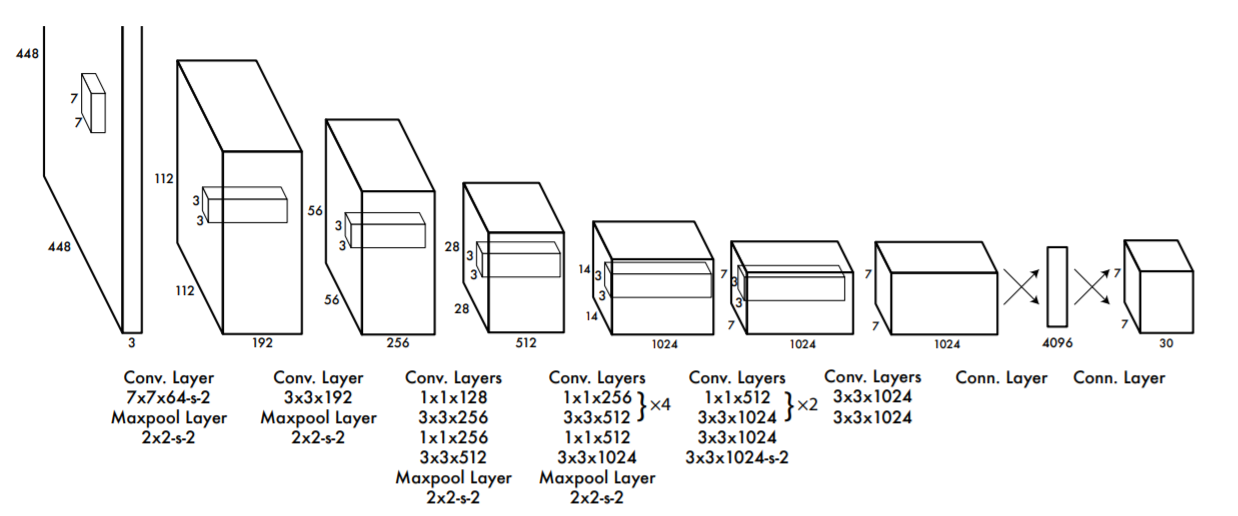
\includegraphics[width=\textwidth]{imagens/yolo.png}
\caption{YOLO Architecture: Simultaneously predicts bounding boxes and class probabilities for these boxes \cite{redmon2016you}}
\label{fig:yolo_arc}
\end{figure}

This architecture makes use of only convolutional neural networks, this topic has been already detailed in Subsection \ref{sec:cnn} and makes it in a fully convolutional network (FCN). Yolo has $75$ convolutional layers, with skip connections and upsampling layers.  





In the YOLO environment, the algorithm divides the input image into a $ZxZ$ grid. And each grid of this frame predicts only one object as is shown in Figure \ref{fig:yolo_flow}. And YOLO uses $7x7$ grids ($ZxZ$), 2 boundary boxes (B) and 20 classes (C). So, the tensor of the YOLO prediction has a shape of $(Z,Z, Bx5+20) = (7,7,30)$


\begin{figure}[H]
\centering
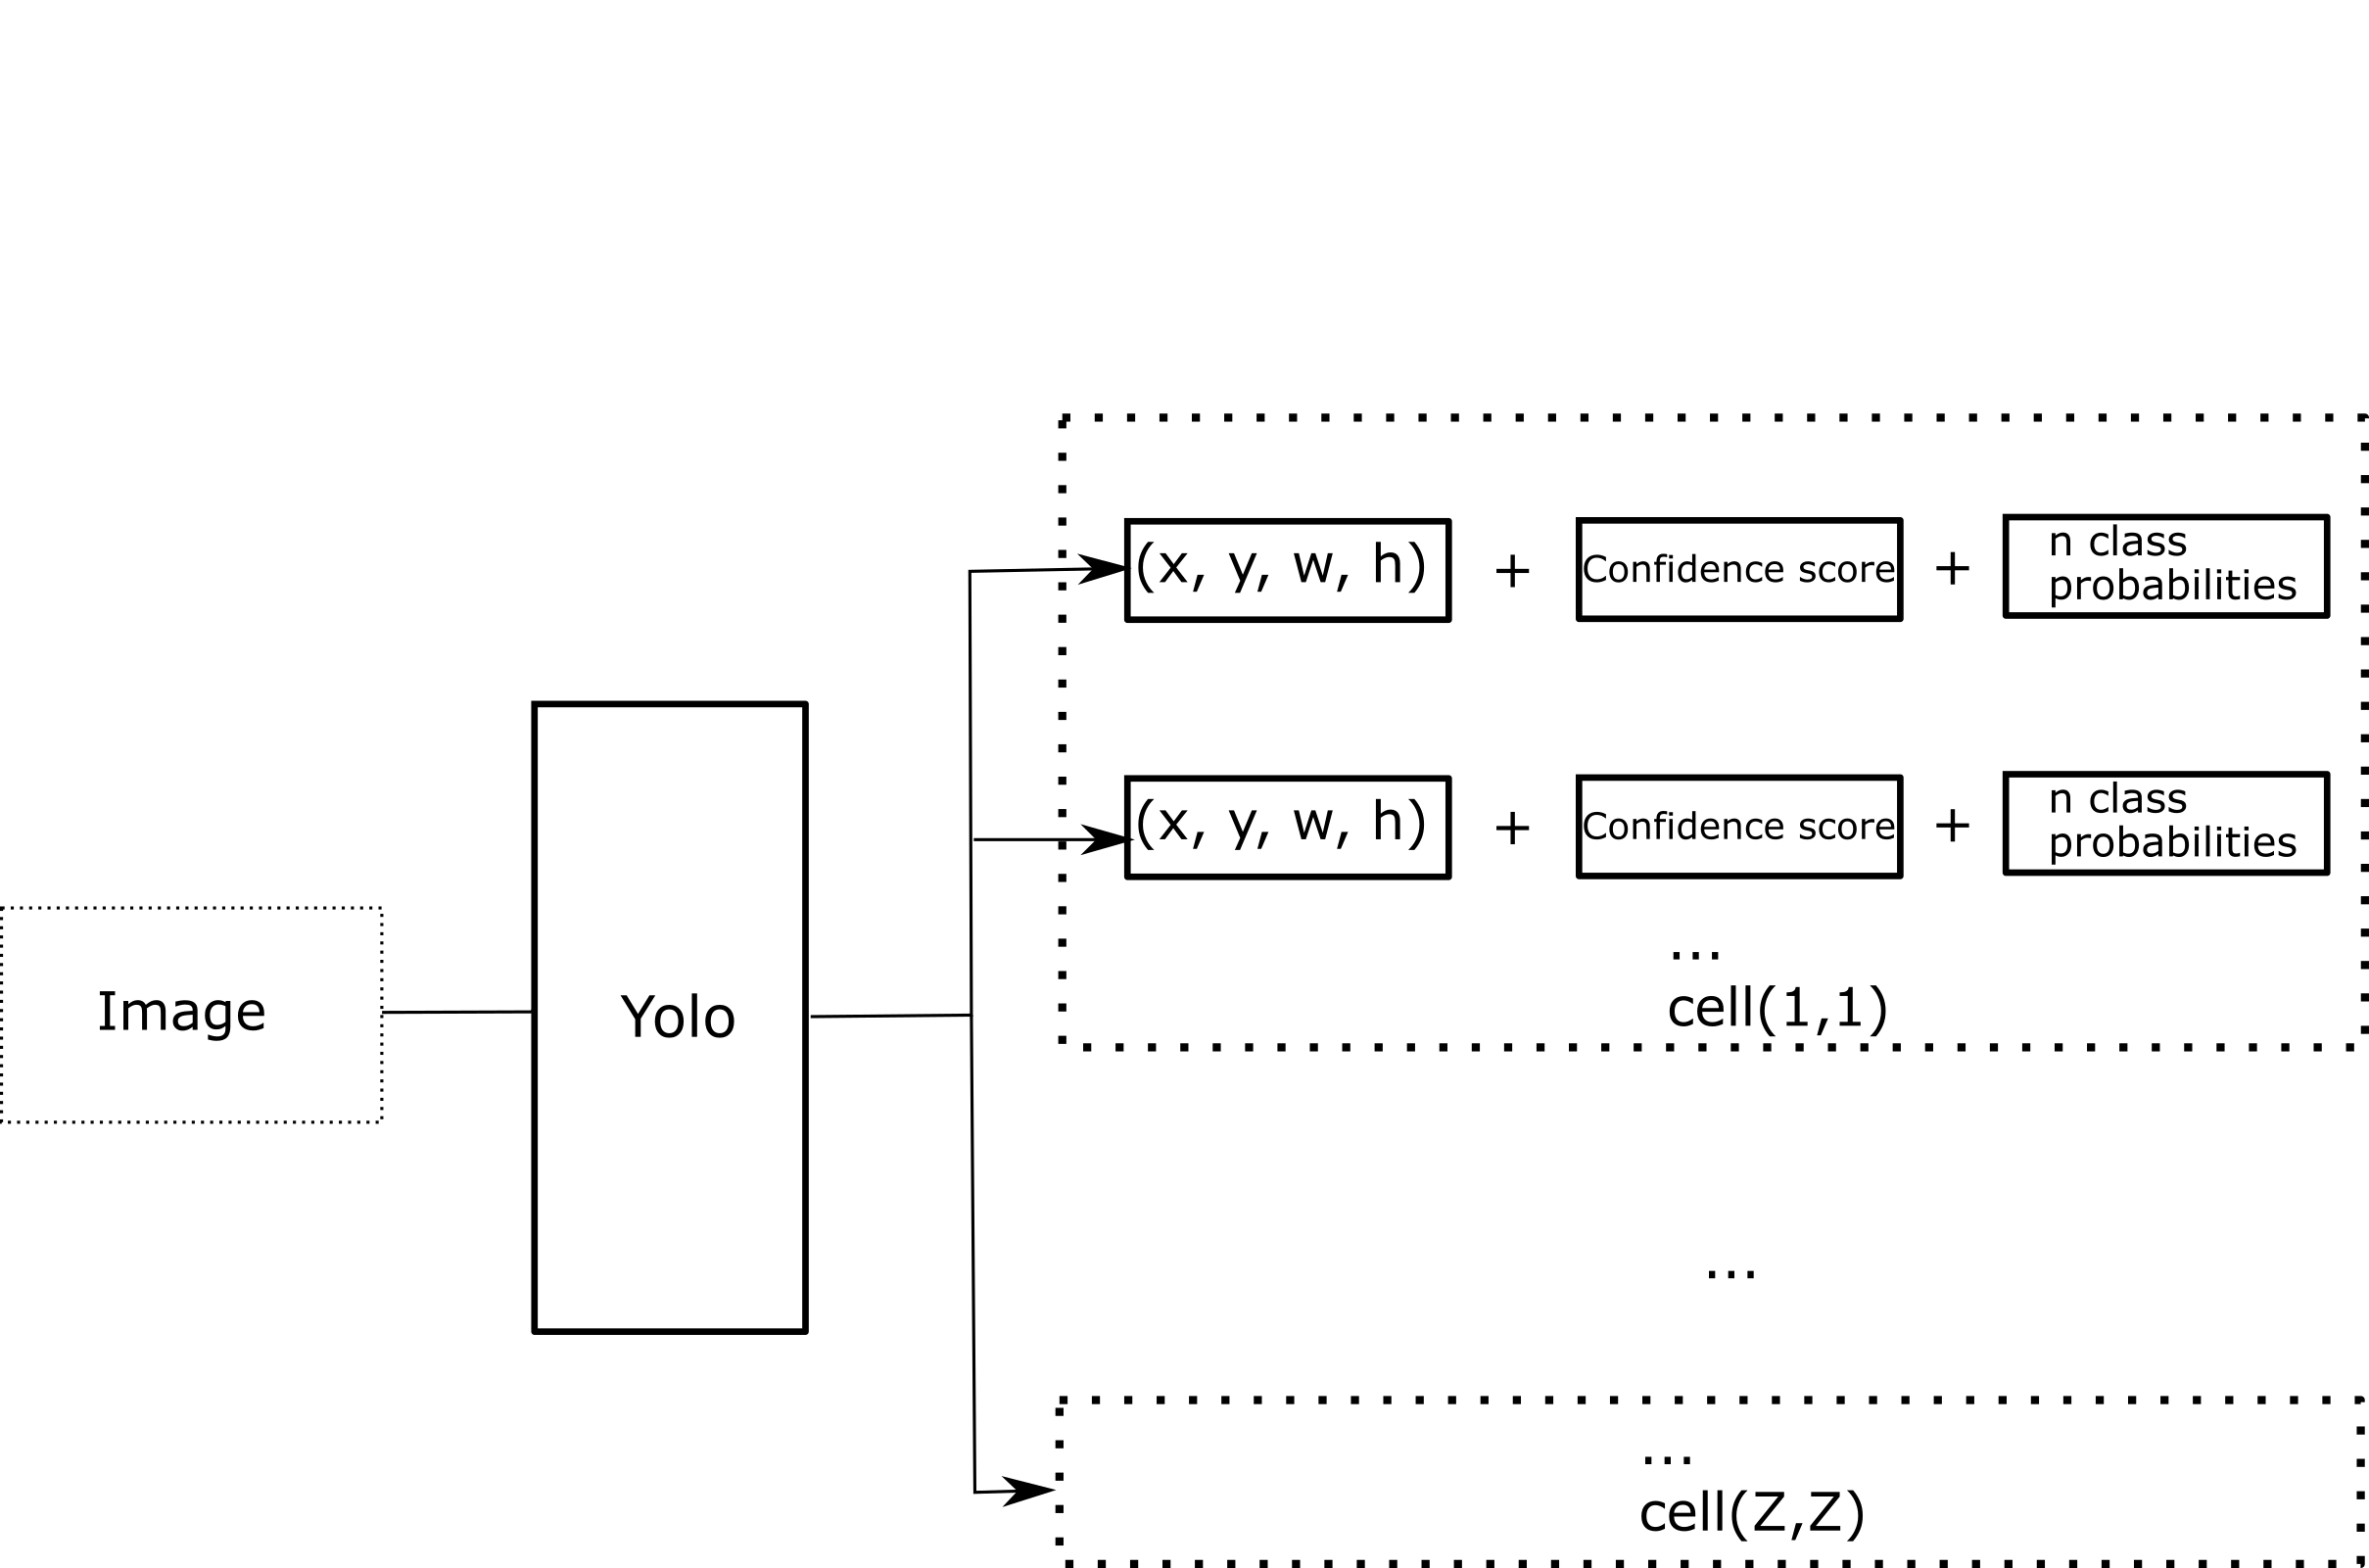
\includegraphics[width=\textwidth]{imagens/yolo_flow.png}
\caption{Yolo makes ZxZ predictions with B boundaries boxes}
\label{fig:yolo_flow}
\end{figure}

Going deeper in the architecture, the object detection is based on the boundary box approach, and each box has 5 known elements (x, y, w, h) and a box confidence score. This score means how likely the box contains an object. It uses a CNN to reduce the spatial dimension, after that it performs a linear regression using two fully connected layers to make the predictions, this approach consider only predictions over 0.5. It is defined in Table \ref{eq:prob_yolo}. 


\begin{table}[H]
\centering
\caption{The Yolo's predicts equations}
\begin{tabular}{l|l} 
\toprule
Description~                   & Equation                                                                 \\
box confidence score           & $P_r(object).IoU$                                                     \\
conditional class probability~ & $P_r(class_i|object)$                                       \\
class confidence score         & $P_r(class_i).IoU$                                                   \\
class confidence score         & box confidence score $\cdot$ conditional class probability  \\
\bottomrule
\end{tabular}
\label{eq:prob_yolo}
\end{table}

where in Table \ref{eq:prob_yolo}, 

$P_r(object)$ is the probability the box contains an object.
$IoU$ is the intersection over the union between the predicted box and the ground truth.
$P_r(class_i|object)$ is the probability the object belongs to $class_i$ given an object is presence.
$P_r(class_i)$ is the probability the object belongs to $class_i$.

The bounding boxes concept is defined in \cite{redmon2017yolo9000}, and in the many problems as in autonomous driving domain, the most common detection will be pedestrian and cars at different distance \cite{ess2010object}. To take care of this problem, it is necessary to apply the clusterization approach, in this case is defined by K-means with $K=5$. Since the algorithm is working with a many kinds of bounding boxes, it is not possible to use the regular spatial distance to measure the data point distances, that is the reason to use $IoU$. Based on the distance of the cluster called as anchor, in this solution will predicts 5 parameters ($t_x, t_y, t_w, t_h,$ and $t_o$) combined with the sigma function to reduce the offset range as is already defined in (\ref{eq:bound}) and it is detailed graphically in Figure \ref{fig:anchor}.


    
    \begin{equation}
    \label{eq:bound}
    \begin{aligned}
        b_x = \sigma(t_x) + c_x \\
        b_y = \sigma(t_y) + c_y \\
        b_w = p_we^{t_w} \\
        b_h = p_he^{t_h} \\
        P_r(object)\cdot IoU(b,object) = \sigma(t_o)
    \end{aligned}
    \end{equation}

where, $t_x, t_y, t_w, t_h$ are the predictions made by the algorithm. 
$c_x, c_y$ are the top left corner of the grid cell of the anchor.
$p_w, p_h$ are the width and height of the anchor. 
$c_x, c_y$ are normalized by the image width and height. 
$b_x, b_y, b_w, b_h$ are the predicted boundary box. 
$\sigma(t_i)$ is the box confidence score.

\begin{figure}[H]
\centering
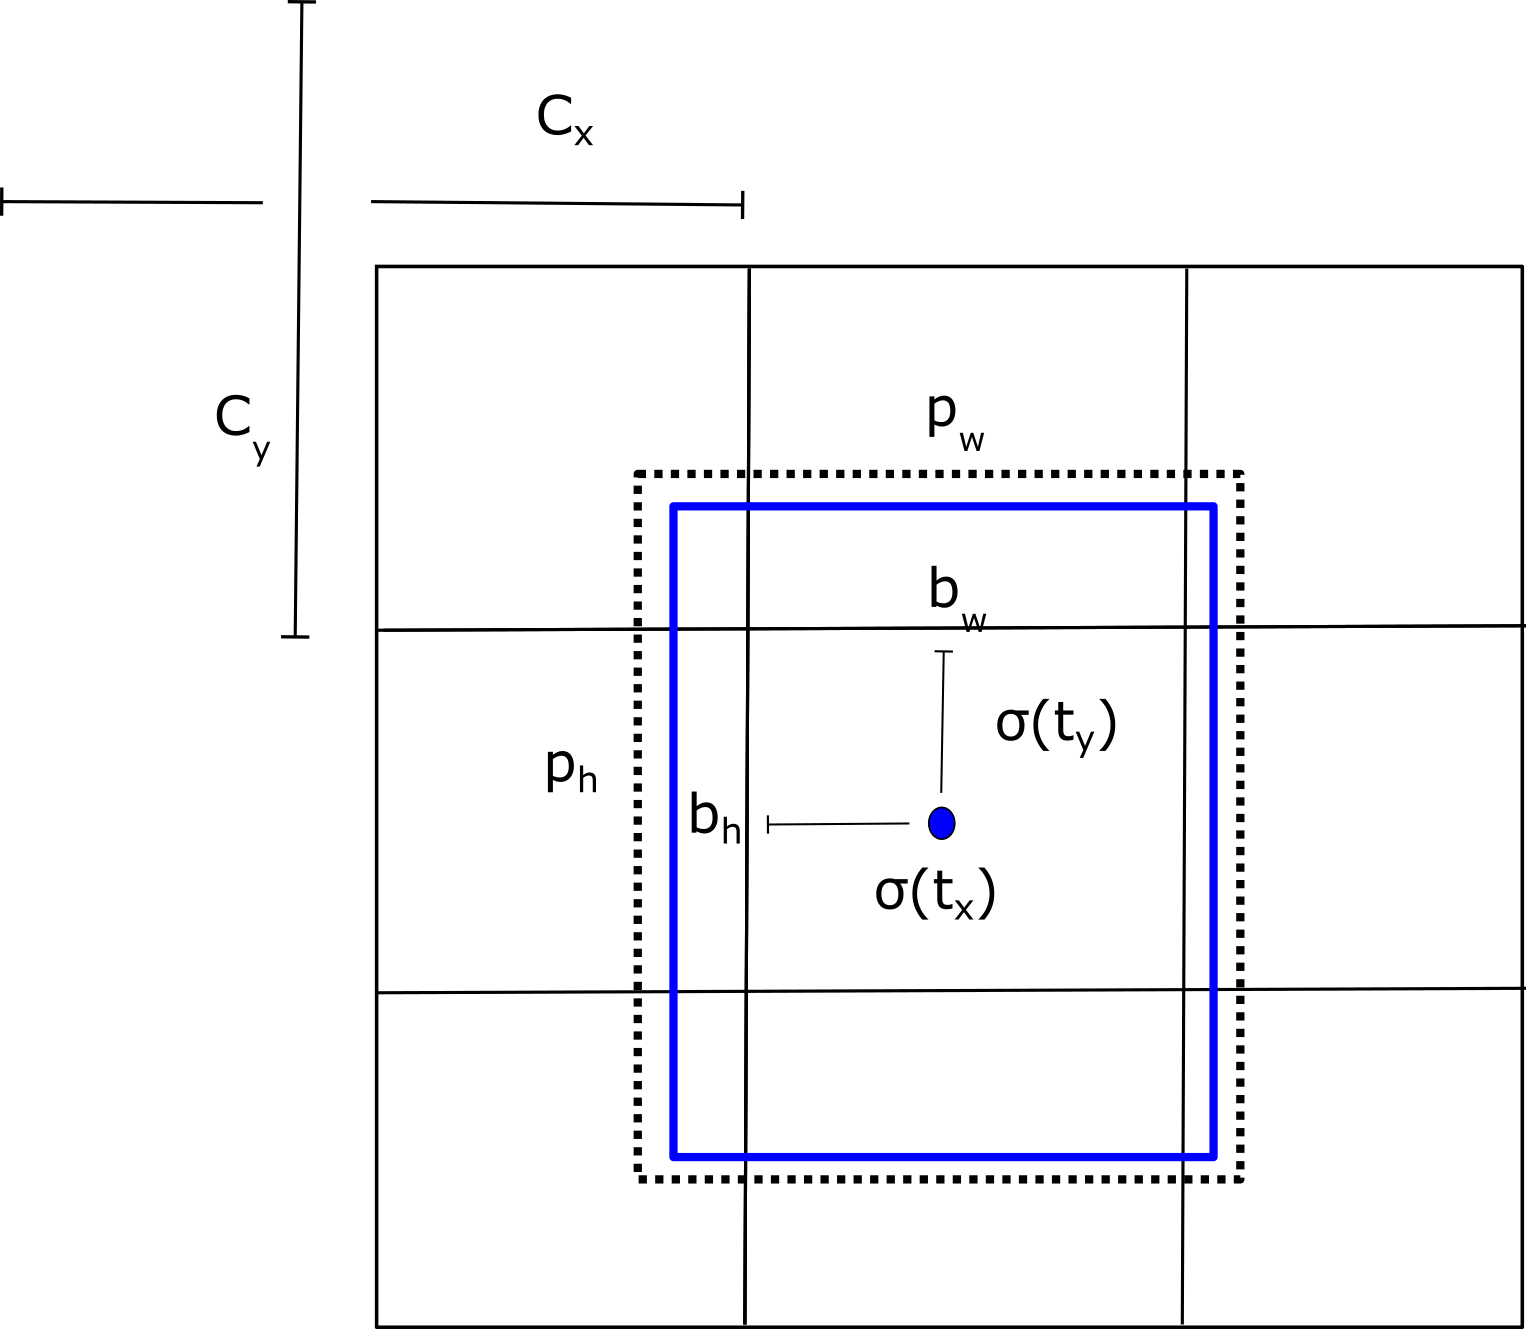
\includegraphics[scale=0.5]{imagens/anchor.png}
\caption{Prediction of the width and height of the box as offsets from clusters centroids based on \cite{redmon2017yolo9000}}
\label{fig:anchor}
\end{figure}

As it already defined, the proposed solution predicts multiple bounding boxes per grid cell. For this is necessary compute the loss for the true positive, with the intention to reduce the error, hence the object is to be faster not accurated, in other hands each cell will be looked on time along the use, and it will be used the highest IoU. The loss funcion is composed by classification loss in (\ref{eq:classification_loss}), the localization loss in (\ref{eq:localization_loss}), the confidence loss (\ref{eq:confidence_loss}), and the loss funtcion is (\ref{eq:loss}). 

If the object is located on the frame, the classification loss will perform the squared error at each cell on the conditional probability for each class: 

\begin{equation}
\label{eq:classification_loss}
    \sum_{i=0}^{s^2}1^{obj}_i \sum_{c\in~classes} \left ( p_i\left ( c \right )-\hat{p}_i\left ( c \right )\right )^2
\end{equation}

where, $1^{obj}_i$ is the boolean that controls if has an object or not, $\hat{p}_i\left ( c \right )$ denotes the conditional probability for each classes in the cell.

The localization loss is necessary to take care about the measure errors regarding the locations and the sizes of the boxes, the goal is not to define the weight absolute errors in large boxes and small boxes, it predicts the square root of the bounding box width and height instead of the width and height. 

\begin{equation}
\label{eq:localization_loss}
\begin{aligned}
    \lambda_{coord}\sum_{i=0}^{s^2}\sum_{j=0}^{B}1^{obj}_i_j\left [ \left ( x_i - \hat{x_i} \right )^2  + (y_i-\hat{y_i})^2 \right ] \\ 
    + \lambda_{coord}\sum_{i=0}^{s^2}\sum_{j=0}^{B}1^{obj}_i_j\left [ \left ( w_i - \hat{w_i} \right )^2  + (h_i-\hat{h_i})^2 \right ] 
    \end{aligned}
\end{equation}

where, $1_{ij}^{obj} = 1$ if the boundary box in the cell is responsible to detect the object, otherwise is 0. $\lambda_{coord}$ increases the weight for the loss in the boundary boxes coordinates, with this variable is possible to put more emphasis on the accuracy, so it is multiplied by the loss, the default value for this work is 5. 

The confidence loss is used to measure the objectness of the box, because a grand part of the boxes do not have any detect object inside, and with this a imbalance issue is noted, to avoid this object is necessary to compute this loss. 

\begin{equation}
    \label{eq:confidence_loss}
    \lambda_{noobj}\sum_{i=0}^{s^2}\sum_{j=0}^{B}1^{noobj}_{ij}\left ( C_i - \hat{C}_i \right )^2
\end{equation}

where, $1^{noobj}_i$ is the complement of $1^{obj}_i$, $\hat{C}_i$ is the box confidence score of the box $j$ in cell $i$, and $\lambda_{noobj}$ takes care of the weights down the loss when a background is detected in this work the used value for this variable is $0.5$. 

The final loss is computed through the add of the previous losses, in (\ref{eq:loss}) is defined the actual loss to reduce the errors in the object detection.

\begin{equation}
\label{eq:loss}
\begin{aligned}
    \lambda_{coord}\sum_{i=0}^{s^2}\sum_{j=0}^{B}1^{obj}_i_j\left [ \left ( x_i - \hat{x_i} \right )^2  + (y_i-\hat{y_i})^2 \right ] \\ 
    + \lambda_{coord}\sum_{i=0}^{s^2}\sum_{j=0}^{B}1^{obj}_i_j\left [ \left ( w_i - \hat{w_i} \right )^2  + (h_i-\hat{h_i})^2 \right ] \\
+    \sum_{i=0}^{s^2}\sum_{j=0}^{B}1^{noobj}_{ij}\left ( C_i - \hat{C}_i \right )^2\\
+  \lambda_{noobj}\sum_{i=0}^{s^2}\sum_{j=0}^{B}1^{noobj}_{ij}\left ( C_i - \hat{C}_i \right )^2\\
+     \sum_{i=0}^{s^2}1^{obj}_i \sum_{c\in~classes} \left ( p_i\left ( c \right )-\hat{p}_i\left ( c \right )\right )^2

    \end{aligned}
\end{equation}

After the object detection, is necessary to perform the object classification, where each box predicts the classes the bounding box, so it is recommend to use multilabel classification. The difference in this work is to use the softmax function in the output of the classifications. The data used in this training is labeled and it was collected from Open Image Dataset \cite{krasin2017openimages}, and this classification was performed over the Darkenet neural network \cite{redmon2013darknet}.

\subsection{Distance Estimation}

For the distance estimation, in this approach is proposed to use the outputs predicted by the object detector, where $4$ variables are predicted, which are $(x, y, w, h)$. In this work, $x,y$ are used to ajust the boundary box, and $w, h$ are used in Figure \ref{fig:yolo_flow} to measure the distance of the object, and these variables will variate according with the distance of the camera. As it was already defined in \cite{cao2013circle} the image will be refracted in the lens and with this is possible to deduce a relationship between the known parameters: focal length $(f)$, distance of the object from the lens $(d)$, distance of the refracted image from the lens $(D)$. In the Figure \ref{fig:distance} is shown how the distance measurer works. 


\begin{figure}[H]
\centering
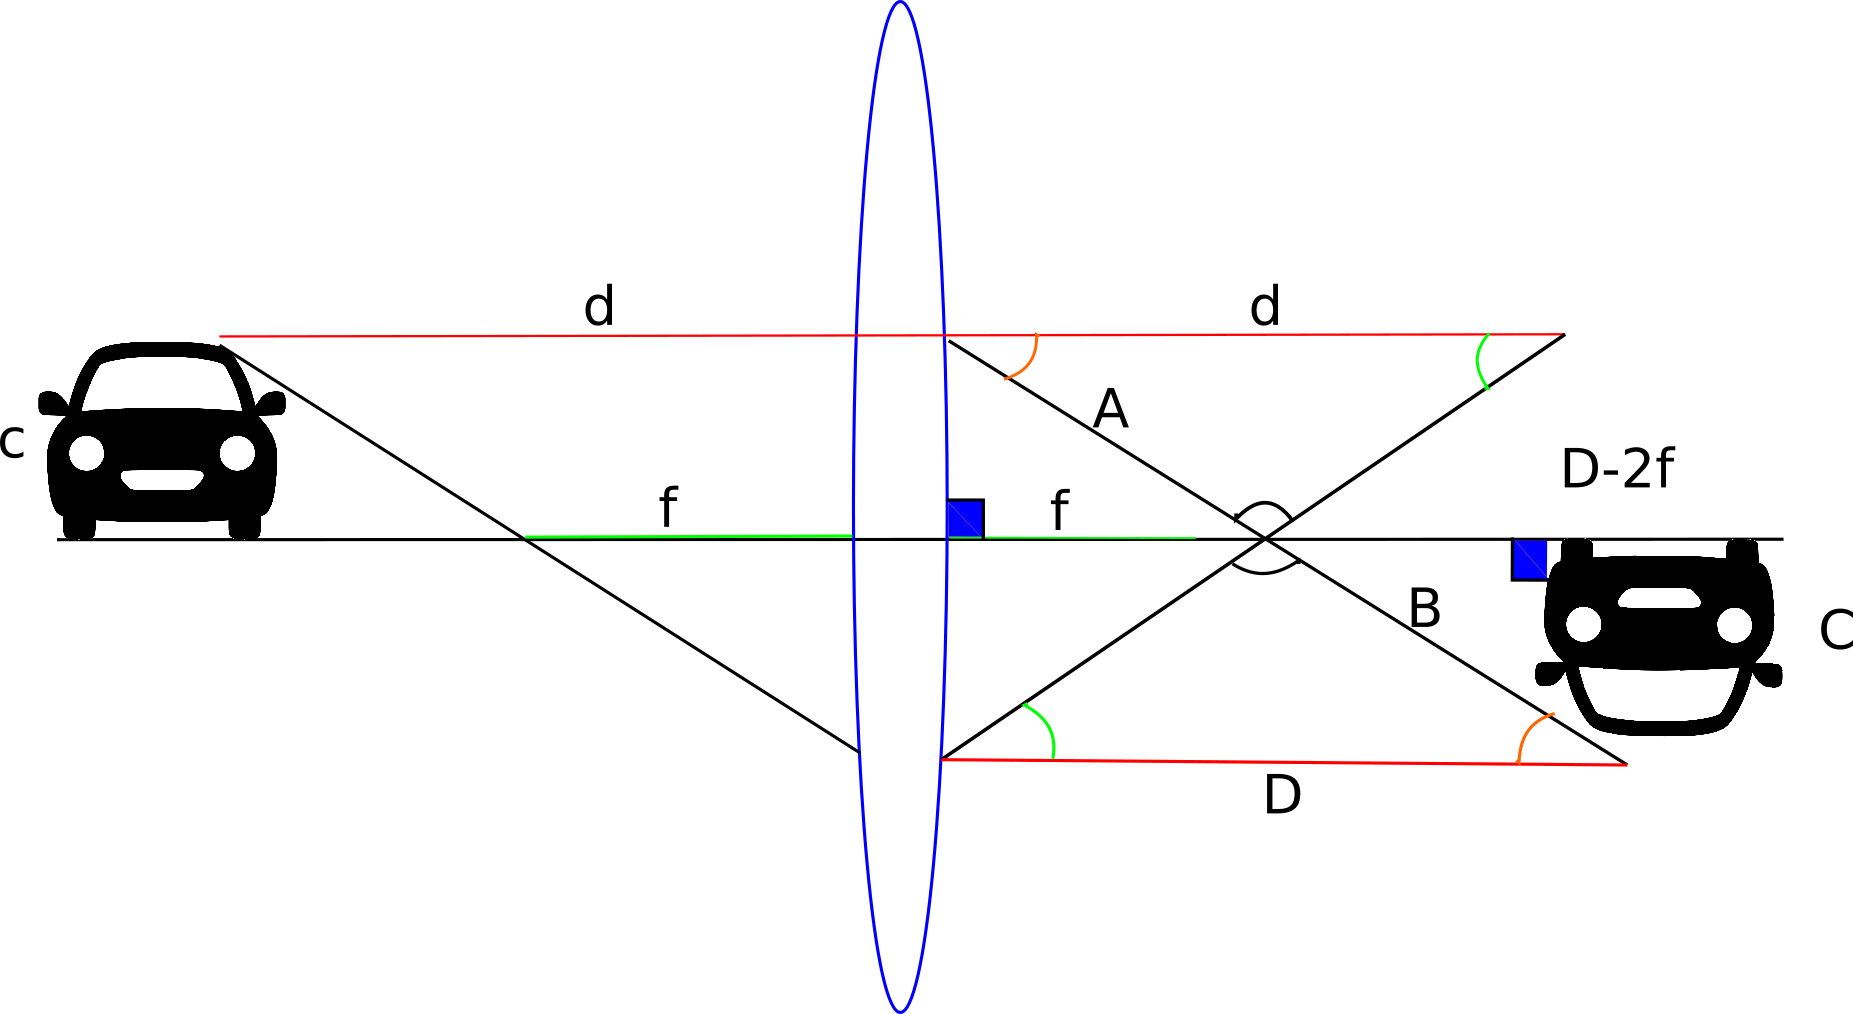
\includegraphics[width=\textwidth]{imagens/desenhando.png}
\caption{Purpose method to compute the distance of the object using cameras}
\label{fig:distance}
\end{figure}


So the red line $d$ represents the actual distance of the object from the convex length. And $D$ gives a sense of how the actual image looks like. Now if we consider a triangle in the left side of the image (new refracted image) with base $d$ and draw a opposite triangle similar to the left side one. So the new base of the opposite triangle will also be do with the same perpendicular distance. Now if we compare the two triangles from right side we will see $d$ and $D$ is parallel and the angle that create on each side of both the triangle are opposite to each other. From which we can infer that, both the triangles on the right side is also similar. Now, as they are similar, ratio of the corresponding sides will be also similar. So $\frac{d}{D} = \frac{A}{B}$. Again if we compare between two triangles in right side of the image where opposite angles are equal and one angle of both the triangles are right angle (90°) (dark blue area). So A:B is both hypotenuse of the similar triangle where both triangle has a right angle. So the new equation can be defined as:

    \begin{equation}\label{eq:meausure}
        \frac{d}{D} = \frac{A}{B} = \frac{f}{D-f},
    \end{equation}

 the focal distance is shown in (\ref{eq:focal}), 

\begin{equation}\label{eq:focal}
    \frac{1}{f} = \frac{1}{d} + \frac{1}{D},
\end{equation}

It is necessary to consider the proportion of the size of each images, as is shown in (\ref{eq:proportion}), these variables come from the object detection, as shown in (\ref{eq:distance}).


\begin{equation}
    \label{eq:proportion}
    d = f + \frac{C}{c},
\end{equation}

the focal length is computed by (\ref{eq:focal_length}), 

\begin{equation}
    \label{eq:focal_length}
    f = \frac{2\cdot 3.14 \cdot 180}{360},
\end{equation}

Finally, it is possible to predict the distance based on outputs from the predictor combined with basic physics in (\ref{eq:distance}), where $w$ is the width and $h$ the height of the object.

\begin{equation}
    \label{eq:distance}
    distance = \frac{2 \cdot 3.14 \cdot  180}{w + h \cdot  360}
\end{equation}



 
\section{Approach 2 – One camera with known map}\label{sub:2}

The second proposed approach is based on  \cite{mayer2016large}, where it is necessary to take the photos and label this images \cite{tzutalin6labelimg}, and its output is shown in Table \ref{tab:output_table}, and indicates the position and size of the boundary box as already defined in Figure \ref{fig:anchor}, and the real position of the car on the real scenario, and show in Figure \ref{fig:proposal2} is shown the block diagrams and the proposed approach to predict the distance based on the known map. In this Subsection is defined only the step regarding the estimate position based on the map, because the other steps has been already defined in Section \ref{sub:1}. 


\begin{figure}[H]
\centering
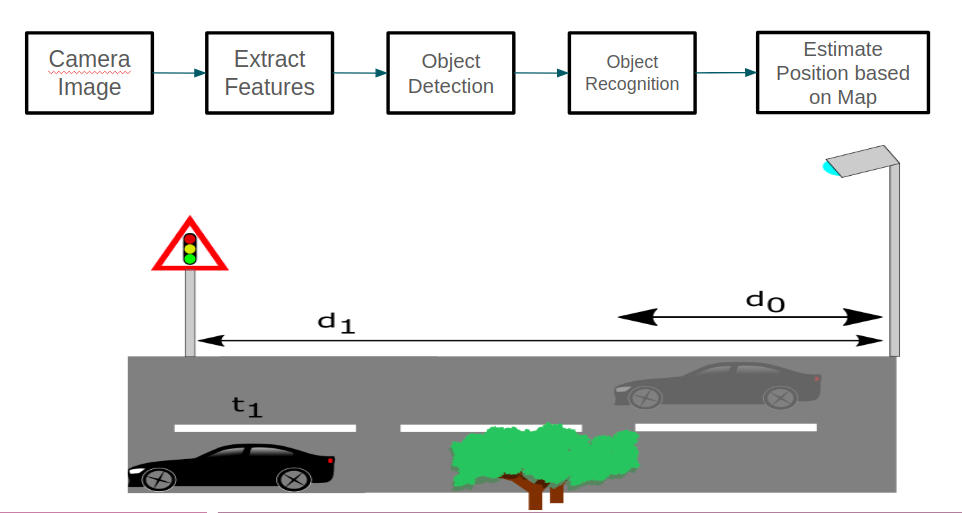
\includegraphics[width=\textwidth]{imagens/proposal2.png}
\caption{Approach using one camera with known map}
\label{fig:proposal2}
\end{figure}


\begin{table}[H]
\centering
\caption{Example of labeled values}
\begin{tabular}{llllll} 
\hline
Label        & Distance (meters) & X    & Y   & W    & H   \\
car #1         & 4.41     & 365  & 304 & 1150 & 563  \\
car #2        & 11.11    & 321  & 256 & 736  & 422  \\
car #3        & 16.24    & 221  & 198 & 562  & 351  \\
car #4        & 19.66    & 138  & 172 & 425  & 296  \\
car #5        & 23.09    & 107  & 150 & 360  & 265  \\
road signal & 25.82    & 1226 & 6   & 1266 & 95   \\
tree        & 17.22    & 507  & 1   & 606  & 231  \\
\hline
\end{tabular}
 \label{tab:output_table}
\end{table}

\subsection{Estimate position based on map}

For this step is necessary to collect data and label of this data before start. Because based on the previous collect data, this predictor will be different compared with the estimation provided in Section \ref{sub:1}. In this approach is used an Artificial Neural Network (ANN), and the concepts of this architecture was defined in 
Subsection \ref{ml-ai}. The proposed ANN is in Figure \ref{fig:rede_neural}.


\begin{figure}[H]
\centering
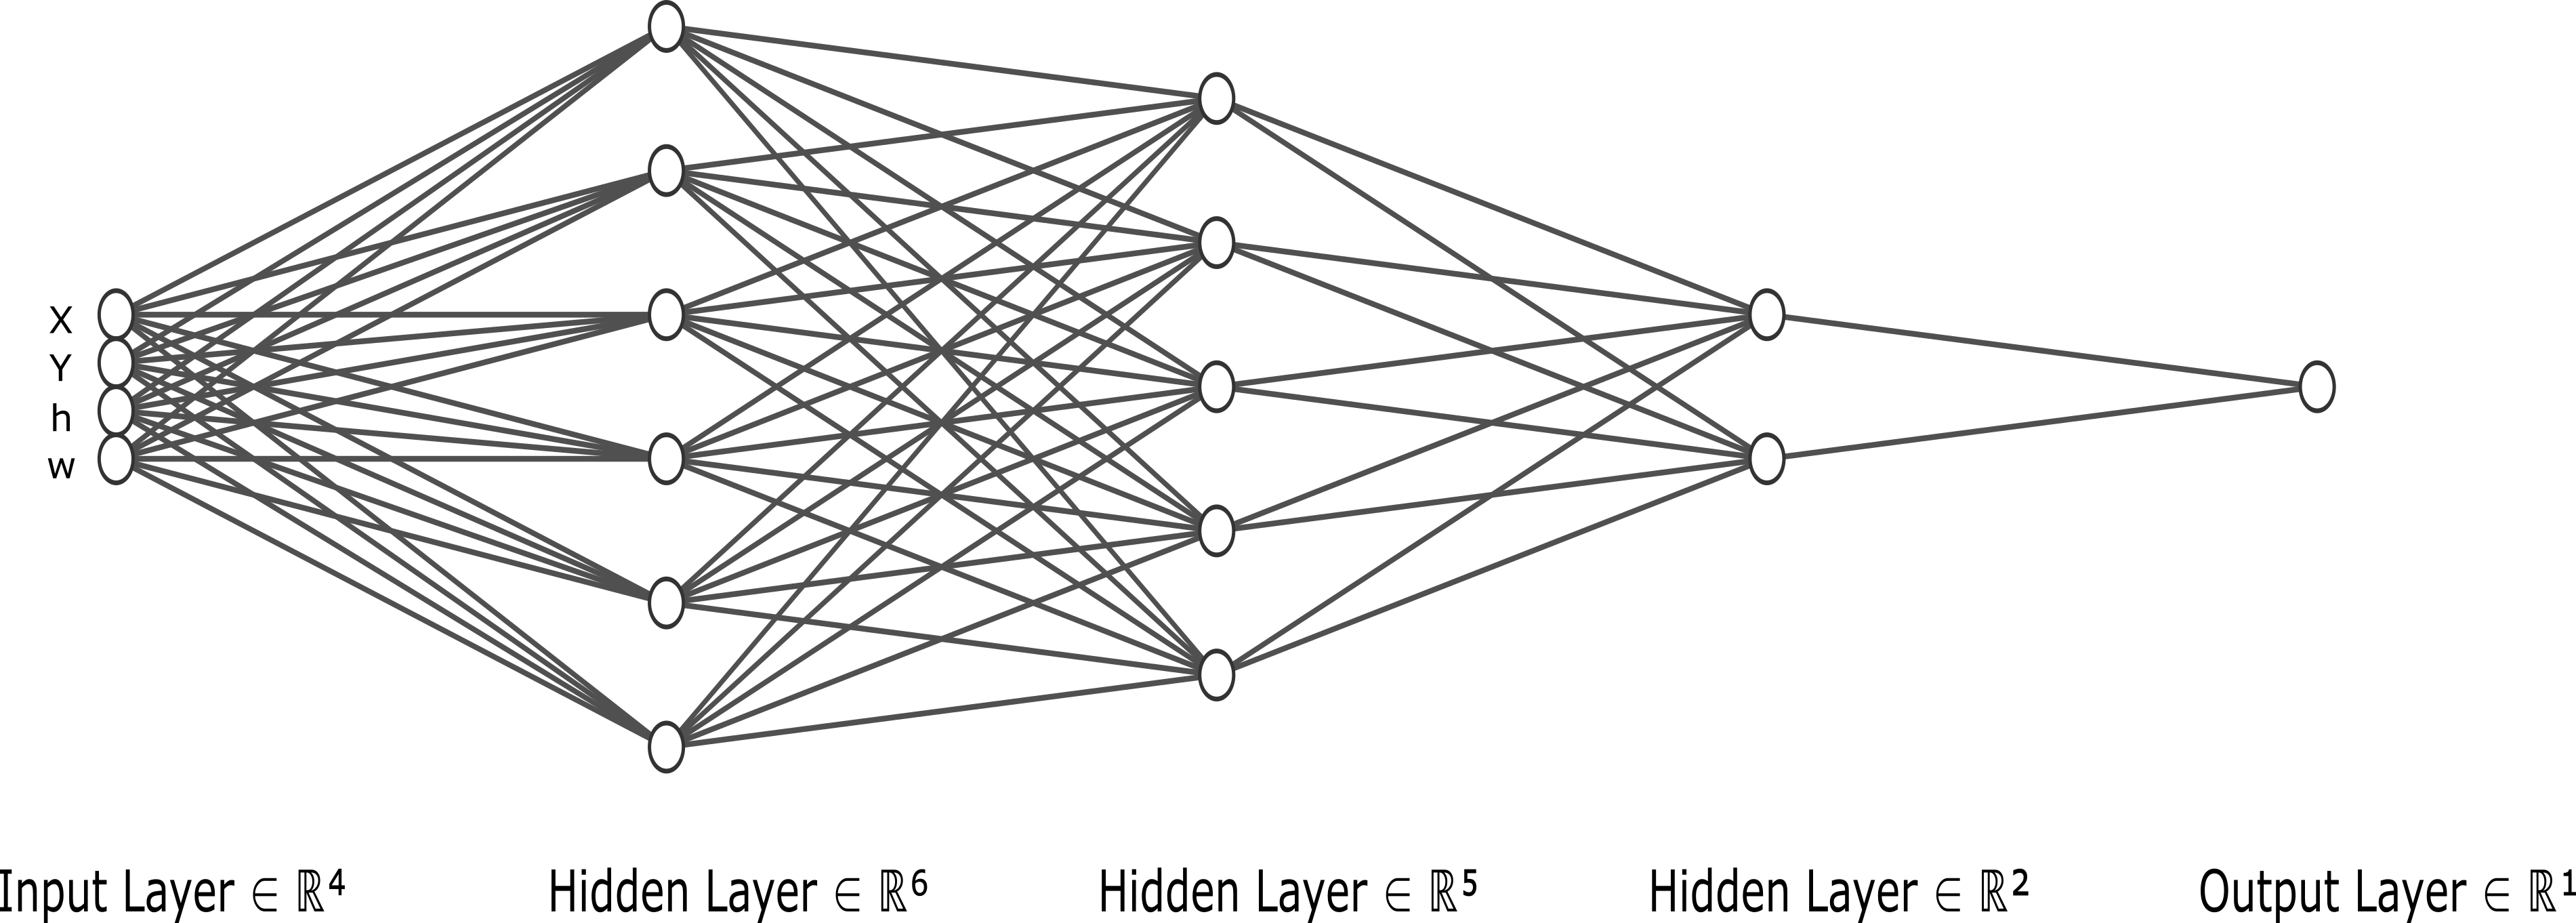
\includegraphics[width=\textwidth]{imagens/nn.png}
\caption{Neural network responsible to predict the distance of the objects based on the boundary boxes}
\label{fig:rede_neural}
\end{figure}

And with this defined architecture is possible to estimate the distance of the car along the scenario, an example of labeled image is shown in Figure \ref{fig:boundary_boxes_car}, these outputs were collected from this image and saved in Extensible Markup Language (XML) file so serve as input in the ANN. 


\begin{figure}[H]
\centering
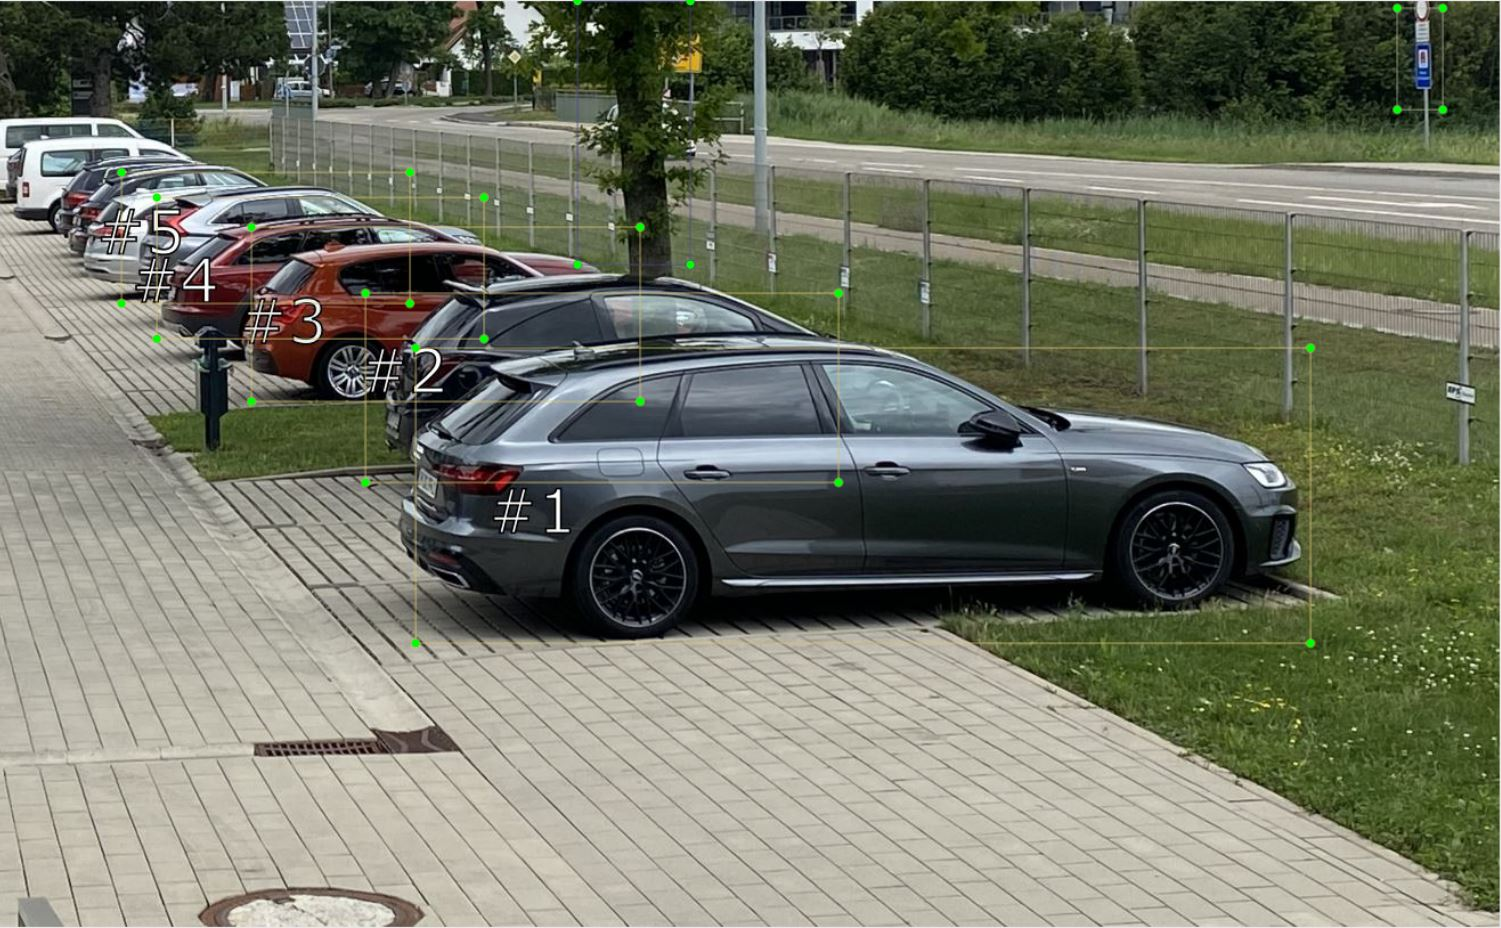
\includegraphics[width=\textwidth]{imagens/boundary_boxes.JPG}
\caption{Labeled image with boundary boxes positioned in each important element of the screen}
\label{fig:boundary_boxes_car}
\end{figure}




\section{Approach 3 – Multicamera}\label{sub:3}

This approach was the selected one for the construction of the framework on Subsection \ref{framework}, because with this approach is possible to consider the position of the camera on the test scenario. As similar in Subsection \ref{sub:2}, only the last step will be defined here, because the another ones were already described in Subsection \ref{sub:1}. 


\begin{figure}[H]
\centering
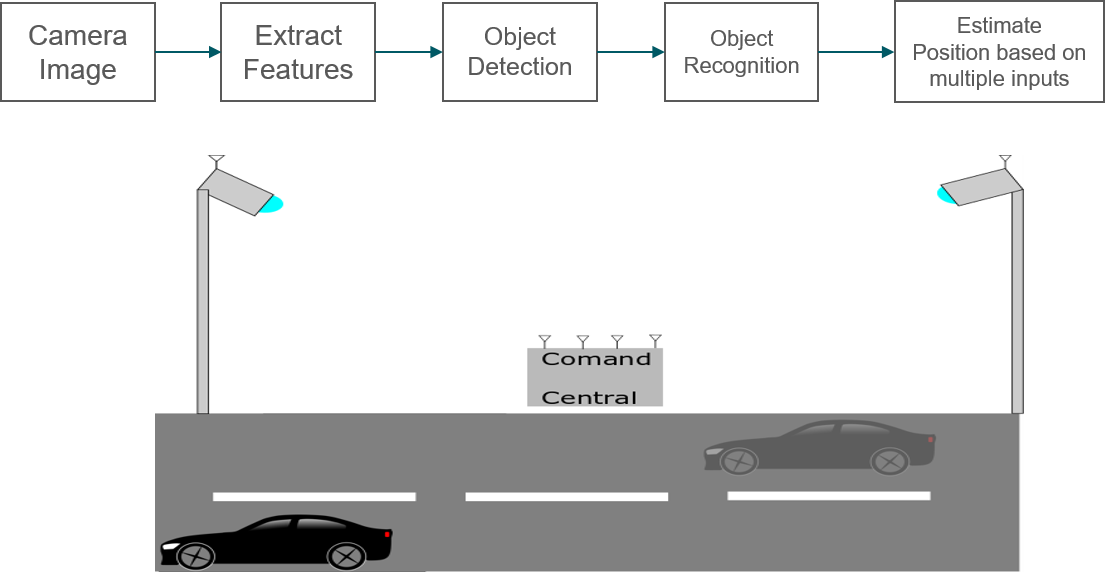
\includegraphics[width=\textwidth]{imagens/proposal3.png}
\caption{Approach using multicamera}
\label{fig:proposal3}
\end{figure}

This approach allow to create a scenario based in multiple cameras and form an array of cameras, and where there is a command central responsible to merge all of collected data and fuse this data on the database such as label of each object, position and its timestamp. 

The data used on this task is provided from streams of the cameras and they send these data to command center via a wireless connection over the protocol IEEE 802.11 and this data fusion is controlled by proxy and it was written in Python. And the distance estimation is based on the Inverse perspective mapping (IPM) and is well defined in \ref{ipm}.


\subsection{Estimate position based on multiple inputs}\label{ipm}
Inverse perspective mapping is a mathematical technique that remove the effects of distortion of a picture when transforming the perspective of the image to another perspective. In spite of disparity mapping, inverse perspective mapping method requires only one camera and this method cannot provide depth information directly ~\cite{Tuohy2010}.

Camera must be located in front of the car with an angle of \(\theta\) to down. Figure \ref{fig:ImageRelationSystem} shows the setup.

\begin{figure}[h]
\centering
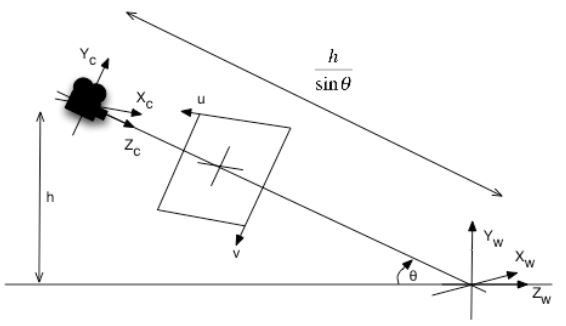
\includegraphics[scale=0.5]{imagens/Inverse Perspective Mapping.JPG}
\caption{Image coordinate system in relation to world coordinate
system.}
\label{fig:ImageRelationSystem}
\end{figure}
\par


This setup was selected based on solution of \cite{Wongsaree2018}, the mathematical background is to create top-down view, the surface road point is known as $(X_w,Y_w,Z_w)$
that projects to the image plane $(u,v)$ is a must. As disrupted in Figure \ref{fig:ImageRelationSystem}. For rotatation angle $(\theta)$, which is angle between camera and the surface, the IPM equation is based on \cite{7759904} and is shown is Equation \ref{eq:eq1}:

\begin{equation}
    (u,v,1)^T = K\cdot T \cdot K (X_w,Y_w, Z_w,1)^T
    \label{eq:eq1}
\end{equation}

where R is the rotation matrix given in the equation \ref{exp2}.
\begin{equation} \label{exp2}
R=
\begin{bmatrix}
1 & 0 & 0 & 0\\
0 & \cos{\theta} & -\sin{\theta} & 0\\
0 & \sin{\theta} & \cos{\theta} & 0\\
0 & 0 & 0 & 1
\end{bmatrix}
\end{equation}
\par

T is the translation matrix given in the equation \ref{exp3}. Where h means the height of the position of the camera.
\begin{equation} \label{exp3}
T=
\begin{bmatrix}
1 & 0 & 0 & 0\\
0 & 1 & 0 & 0\\
0 & 0 & 1 & \frac{-h}{\sin{\theta}}\\
0 & 0 & 0 & 1
\end{bmatrix}
\end{equation}


\par
K is the camera parameter matrix given in the Equation \ref{exp4}. Where $f$ is the focal length of the camera, $s$ is the skew parameter and $u_0, v_0$ are the center of the pixel of desired image size. 
\begin{equation} \label{exp4}
K =
\begin{bmatrix}
f & s & u_0 & 0\\
0 & f & v_0 & 0\\
0 & 0 & 1 & 0\\
\end{bmatrix}
\end{equation}

The Equation \ref{exp4} can be replaced using the real parameters of this test scenario and these parameters are $f = 2.92 mm, s=0, u_0=240, v_0=160$. Replacing the Equations \ref{exp2},\ref{exp3}, \ref{exp4} into the initial Equation \ref{eq:eq1}, achieving the new Equation \ref{eq:eq2}.

\begin{equation}
    \begin{bmatrix}
u\\ 
v\\ 
1
\end{bmatrix}
=\begin{bmatrix}
P_{11} & P_{12} & P_{13} & P_{14}\\ 
P_{21} & P_{22} & P_{23} & P_{24}\\ 
P_{31} & P_{32} & P_{33} & P_{34}
\end{bmatrix}
\begin{bmatrix}
X_w\\ 
Y_w\\ 
Z_w\\
1
\end{bmatrix}
\label{eq:eq2}
\end{equation}

where the matrix P was gotten from product between K, T, and R. As is only necessary to evaluate the position of the road, so the coordinate $Y_w$ can be equal to 0, so simplifying the Equation \ref{eq:eq2}, so it is given by Equation \ref{eq:eq3}.

\begin{equation}
    \label{eq:eq3}
    \begin{bmatrix}
u\\ 
v\\ 
1
\end{bmatrix}
=\begin{bmatrix}
P_{11} & P_{12}  & P_{14}\\ 
P_{21} & P_{22}  & P_{24}\\ 
P_{31} & P_{32}  & P_{34}
\end{bmatrix}
\begin{bmatrix}
X_w\\ 
Z_w\\
1
\end{bmatrix}
\end{equation}

Based on the Equations above, it is possible to infer the Equation \ref{eq:eq4} for compute the distance from the camera until the object. 

\begin{enumerate}
    \item Calculating average intensity in row direction from bottom row up to top row
    \item The average intensity of each row is compared with the threshold level (obtained from the experimental) which is 50. The starting position of an object is indicated if the average intensity in that row is greater than 50 and the order of that row is stored in a parameter p.
    \item The distance between object and vehicle is therefore calculated using a linear equation given in \ref{eq:eq4}.
\end{enumerate}

\begin{equation}
    \label{eq:eq4}
    d = ap+b
\end{equation}

where $d$ is distance between camera and object and vehicle in meter, $p$ is the order of the row that object is detected and $a, b$ are constants.

 
\section{Framework Architecture} \label{framework}

In this section is discussed how the architecture of the Subsection \ref{sub:3} is encapsulated in a software framework. This Architecture was divided in four big modules: client, model, proxy, and controller. 



\begin{figure}[H]
\centering
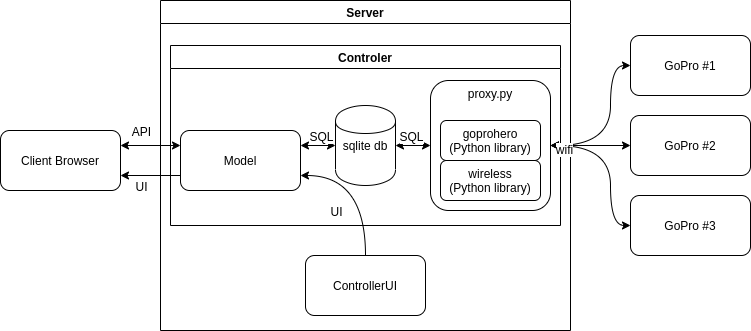
\includegraphics[scale=0.6]{imagens/diagram.png}
\caption{Architecture approach of framework}
\label{fig:framework}
\end{figure}

The first module is the block 1 of Figure \ref{fig:framework} is the client which is responsible to permit all of the interactions with the user and allow to see the cameras doing the inference and see the boundary boxes and the labels, and the distance estimation as well.

The module responsible to control the model is the block 2 of Figure \ref{fig:framework} and it will be expanded in Figure \ref{fig:networkBehavior}. The input data is gotten from data provided from cameras and the output will be saved in the database, these outputs have already defined in Section \ref{sub:3}. 

The block 3 of Figure \ref{fig:framework} needs to control all of this flow along the usage of this framework and provide an abstraction layer to the usage of the database. 

In block 4 of Figure \ref{fig:framework} is the part responsible to connect the other cameras via WIFI protocol and allows the system to connect another cameras, the total amount of camera is based on the hardware available for the tests. 


In Figure \ref{fig:networkBehavior} is shown how the model performs the inference process along the detection time.  

\begin{figure}[H]
\centering
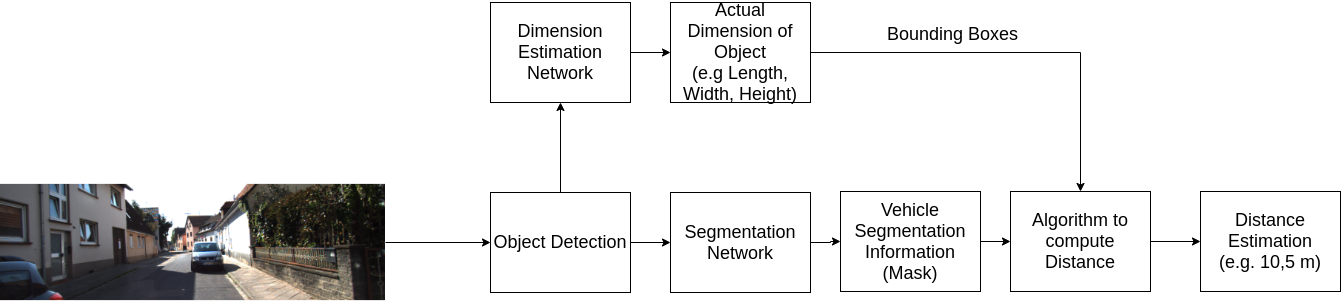
\includegraphics[width=\textwidth]{imagens/Network Behavior.png}
\caption{Architecture of framework based on multicameras perspective}
\label{fig:networkBehavior}
\end{figure}